% This file was created with tikzplotlib v0.9.12.
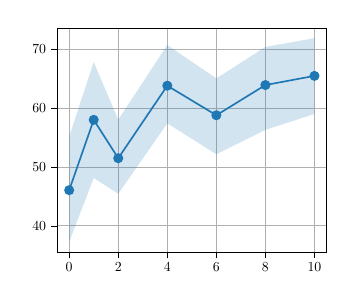
\begin{tikzpicture}[scale=0.5]

\definecolor{color0}{rgb}{0.12156862745098,0.466666666666667,0.705882352941177}

\begin{axis}[
tick align=outside,
tick pos=left,
x grid style={white!69.0196078431373!black},
xmajorgrids,
xmin=-0.5, xmax=10.5,
xtick style={color=black},
y grid style={white!69.0196078431373!black},
ymajorgrids,
ymin=35.5108475833333, ymax=73.6249474166667,
ytick style={color=black}
]
\path [fill=color0, fill opacity=0.2]
(axis cs:0,55.1472116666667)
--(axis cs:0,37.2433066666667)
--(axis cs:1,48.1075983333333)
--(axis cs:2,45.4322233333333)
--(axis cs:4,57.4046316666667)
--(axis cs:6,52.1457733333333)
--(axis cs:8,56.3026916666667)
--(axis cs:10,58.9981916666667)
--(axis cs:10,71.8924883333333)
--(axis cs:10,71.8924883333333)
--(axis cs:8,70.39101)
--(axis cs:6,65.047115)
--(axis cs:4,70.7218733333333)
--(axis cs:2,58.02641)
--(axis cs:1,67.8304316666667)
--(axis cs:0,55.1472116666667)
--cycle;

\addplot [very thick, color0, mark=*, mark size=3, mark options={solid}]
table {%
0 46.0402381666667
1 58.0000413333333
2 51.474448
4 63.805701
6 58.7812183333333
8 63.9189143333333
10 65.4759335
};
\end{axis}

\end{tikzpicture}
